\section{Struktur Arduino}
\subsection{Pengertian Arduino UNO}
\begin{figure}[!htbp]
  \centering
  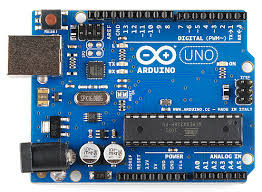
\includegraphics[width=.75\textwidth]{figures/Arduino/arduinouno.jpg}
  \caption{Ini adalah Arduino UNO}\label{fig:arduinouno}
\end{figure}
Arduino (pada gambar \ref{fig:arduinouno}) adalah pengendali mikro single-board yang bersifat open-source, diturunkan dari Wiring platform, dirancang untuk memudahkan penggunaan elektronik dalam berbagai bidang. Arduino UNO merupakan sebuah board mikrokontroler yang dikontrol penuh oleh ATmega328.

\subsection{Kegunaan Arduino UNO}
Arduino dapat disambungkan dan mengontrol led, beberapa led, bahkan banyak led, motor DC, relay, servo, modul dan sensor-sensor, serta banyak lagi komponen lainnya.

\section{Digital Analog}
Perintah navigasi direktori

\section{IDE}
IDE adalah software yang berperan dalam menulis, meng-\textit{compile} program menjadi kode biner dan meng-\textit{upload} ke dalam \textit{memory} microcontroller \cite{djuandi2011pengenalan}. Software IDE (\textit{Integrated Development Environment}) seperti pada gambar \ref{fig:IDE}.
\begin{figure}[!htbp]
  \centering
  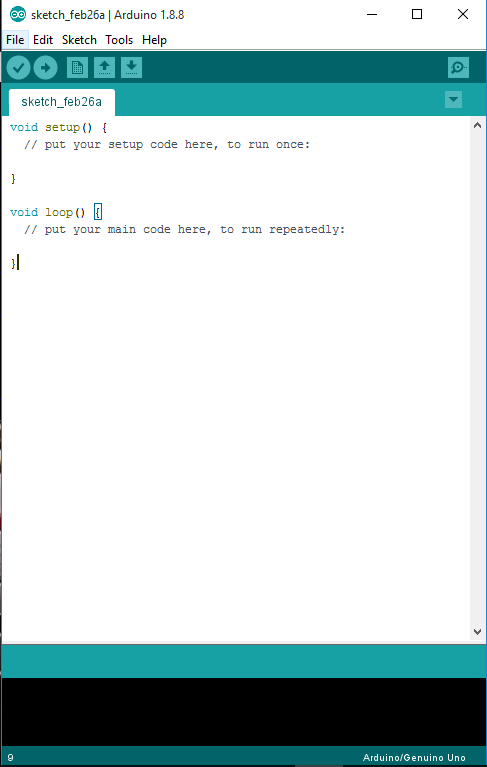
\includegraphics[width=.75\textwidth]{figures/Arduino/IDE.png}
  \caption{Ini adalah Software IDE}\label{fig:IDE}
\end{figure}

\section{Membuat Rancangan Rangkaian}
    Membuat rangkaian dapat dilakukan dengan bantuan aplikasi simulator contohnya VBB (Virtual Bread Board).
\begin{figure}[!htbp]
  \centering
  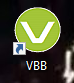
\includegraphics[width=.45\textwidth]{figures/VBB/vbb.png}
  \caption{Ini adalah aplikasi VBB}\label{fig:vbb}
\end{figure}

Bagaimana cara install VBB?
\begin{enumerate}
\item Download installer vbb

\item Double-click installer vbb,seperti pada gambar \ref{fig:installer}
\begin{figure}[!htbp]
  \centering
  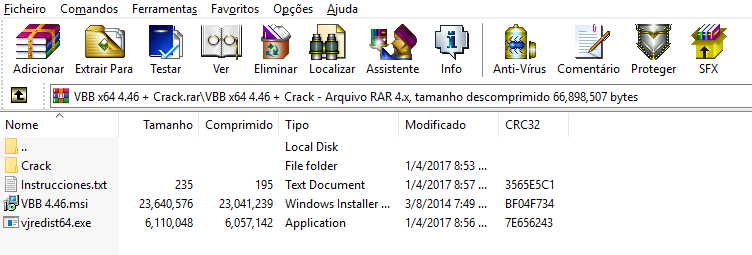
\includegraphics[width=.75\textwidth]{figures/VBB/installer.png}
  \caption{Ini adalah installer}\label{fig:installer}
\end{figure}

\item Maka akan tampil seperti gambar \ref{fig:halawalinstallasi}
\begin{figure}[!htbp]
  \centering
  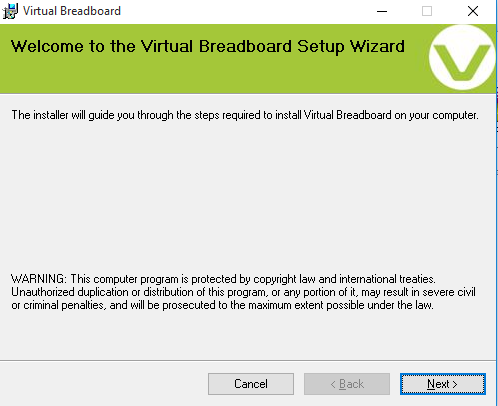
\includegraphics[width=.75\textwidth]{figures/VBB/halawalinstallasi.png}
  \caption{Ini adalah Halaman Awal Installasi}\label{fig:halawalinstallasi}
\end{figure}

\item Pilih direktori penyimpanan seperti gambar \ref{fig:memilihdirektori}
\begin{figure}[!htbp]
  \centering
  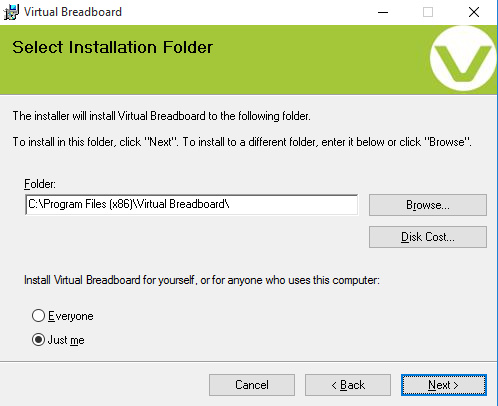
\includegraphics[width=.75\textwidth]{figures/VBB/memilihdirektori.png}
  \caption{Ini adalah Halaman Pemilihan Direktori}\label{fig:memilihdirektori}
\end{figure}


\item Kemudian tekan tombol next, maka akan muncul halaman konfirmasi seperti pada gambar \ref{fig:konfirmasiinstall}
\begin{figure}[!htbp]
  \centering
  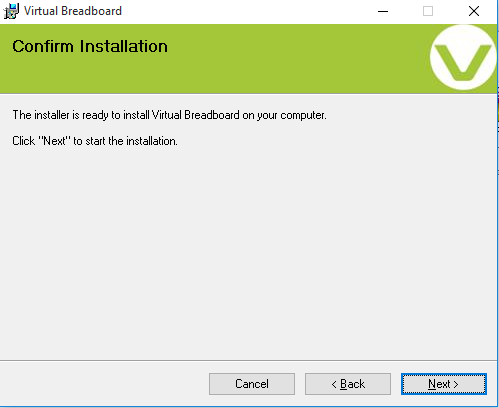
\includegraphics[width=.75\textwidth]{figures/VBB/konfirmasiinstall.png}
  \caption{Ini adalah Halaman Konfirmasi Installasi}\label{fig:konfirmasiinstall}
\end{figure}

\item Lalu tunggu sampai proses installasi selesai, seperti pada gambar \ref{fig:prosesinstallasi}
\begin{figure}[!htbp]
  \centering
  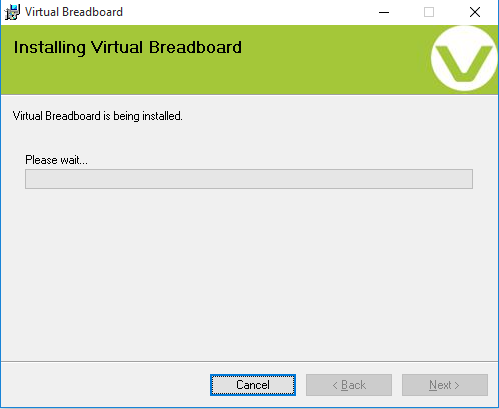
\includegraphics[width=.75\textwidth]{figures/VBB/prosesinstallasi.png}
  \caption{Ini adalah Proses Installasi}\label{fig:prosesinstallasi}
\end{figure}

\item Proses installasi selesai, seperti pada gambar \ref{fig:installasiselesai}
\begin{figure}[!htbp]
  \centering
  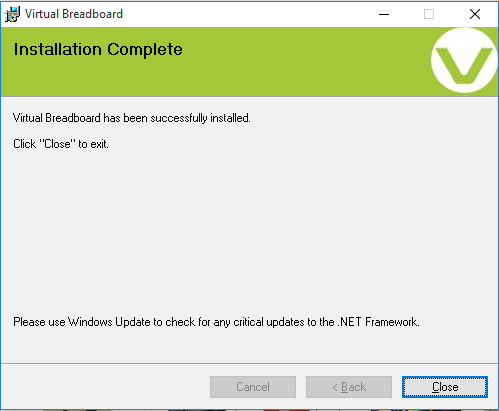
\includegraphics[width=.75\textwidth]{figures/VBB/installasiselesai.png}
  \caption{Ini adalah Proses Installasi Telah Selesai}\label{fig:installasiselesai}
\end{figure}
\end{enumerate} 